\subsection{Lange und kurze Spule}
Bei diesem Teil des Versuchs sollen die Magnetfelder $B$ von einer langen und einer kurzen Spule bei konstantem Strom in Abhängigkeit 
des Abstands $x$ ermittelt werden.
Die Werte für beide Spulen werden jeweils in einem $x$-$B$-Diagramm in Abschnitt \ref{sec:kurze_und_lange_Spule} dargestellt.
Es steht eine longitudinale Hall-Sonde zur Verfügung, die je nach Spule mittels eines Statives in der Höhe angepasst werden muss, 
sodass sie mittig von der Spule ist.
Das Leiterplättchen ist dabei auf der rechten Seite der Sonde.
Außerdem ist an dem Tisch eine Messlatte angeklebt, sodass die Abstände bestimmt werden können.
Für beide Messungen wird die Sonde bei der $\qty{50}{\cm}$ Marke des Lineals aufgestellt und die Spulen werden verschoben.
Das hat den Vorteil, dass die beiden gewählten Spulen jeweils auf bzw. in einem \enquote{Quader} montiert sind (vgl. abbildung \ref{fig:lange_kurze_spule}), 
die längs des Lineals verschoben wird,  sodass keine ungewollten Verschiebungen oder Rotationen geschehen, wenn der eigentliche Abstand geändert wird.
Es werden Spannungsgerät bzw. Spule und die Sonde verkabelt.

\noindent
Die Spulen werden so weit wie möglich über die Sonde geschoben und die Position des linken Randes der Spule wird am Lineal abgelesen.
Um den Abstand von der Sonde zu der Spule besser darstellen zu können wird die $x$ Achse so gelegt, 
dass $x = 0$ ist, wenn die Sonde in der Mitte der Spule ist.
Danach wird der Abstand in unterschiedlichen Abständen erhöht und Messwerte innerhalb und außerhalb der Spulen aufgenommen.

% Die Spule wird anschließend so weit wie es geht nach links über die Sonde gezogen und mit einem konstanten Strom betrieben.
% Die Position des linken Rands der Spule $x_\text{absolut}$ wird an der Messlatte abgelesen.
% Um den Abstand von der Sonde zu der Spule besser darstellen zu können wird die $x$ Achse so gelegt, 
% dass $x = 0$ ist, wenn die Sonde in der Mitte der Spule ist.
% Für die Transformation gilt also bei der langen Spule $x = x_\text{absolut} - \qty{50}{\cm} + \qty{8}{\cm}$ 

\begin{figure}
    \centering
    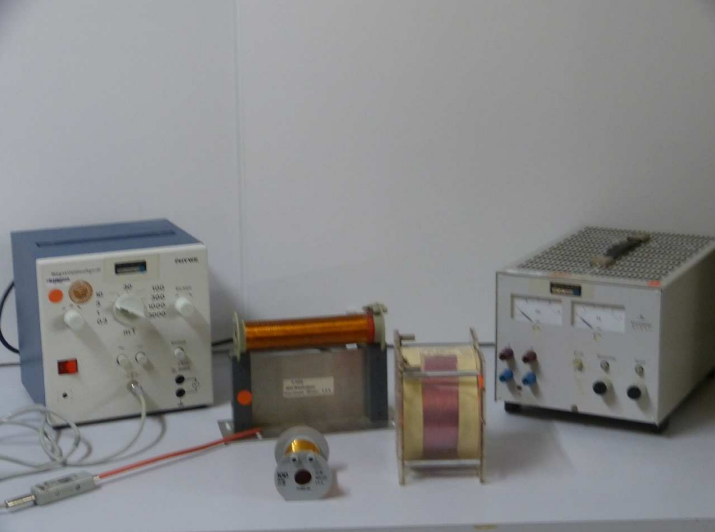
\includegraphics[height = 7cm]{abbildungen/lange und kurze spule.png}
    \caption[]{Versuchsaufbau zur langen und zur kurzen Spule \cite[]{man:v308}.}
    \label{fig:lange_kurze_spule}
\end{figure}

\subsubsection{Die kurze Spule}
Die kurze Spule hat die Windungszahl $n = 3400$, die Länge $l = \qty[]{9}{\cm}$, sowie einen Außendurchmesser von 
$D_\text{außen} = \qty[]{13}{\cm}$ und einen Innendurchmesser von $D_\text{innen} = \qty[]{8.5}{\cm}$.
Die Längen werden jeweils mit dem Maßband bestimmt und die Windungszahl der Spulenbeschriftung entnommen.
Die Stromstärke $I$ beträgt \qty[]{0.6}{\ampere} und die Spannung $U = \qty[]{40}{\volt}$.


\subsubsection{Die lange Spule}
Nach der Anleitung \cite[]{man:v308} beträgt die Windungszahl der langen Spule $n = 300$ und der mittlere Spulendurchmesser $D = \qty[]{41}{\mm}$.
Die Länge $l$ wird mit dem Maßband zu \qty[]{16}{cm} vermessen.
Anschließend wird der Strom auf $I = \qty[]{1}{\ampere}$ und die Spannung auf $U = \qty[]{3.5}{\volt}$ reguliert.
